
%(BEGIN_QUESTION)
% Copyright 2011, Tony R. Kuphaldt, released under the Creative Commons Attribution License (v 1.0)
% This means you may do almost anything with this work of mine, so long as you give me proper credit

Calculate the amount of force exerted by each piston as they receive hydraulic oil pressure from a common pump.   Assume a large piston diameter of 4.83 inches and a small piston diameter of 0.47 inches:

$$\includegraphics[width=15.5cm]{i03462x01.eps}$$

\underbar{file i03462}
%(END_QUESTION)





%(BEGIN_ANSWER)

\noindent
5 points each answer:

\vskip 10pt

Left (large) piston = 17,626 pounds \hskip 30pt Right (small) piston = 166.9 pounds

%(END_ANSWER)





%(BEGIN_NOTES)

{\bf This question is intended for exams only and not worksheets!}.

%(END_NOTES)


